\chapter{Track B: the class LoRA}
\label{ch:trackB}

Track~B asks: \emph{does a small amount of task-specific training change what Qwen2-VL-2B can do?} It was first run on 29 September with the full card (67.3\,\%), and re-run properly on 20 October with balanced training patches and the label-free card (36.4\,\%). The second run is the one to report.

\section{The reported run: balanced and leak-free (Ada job 29575)}

\begin{wherecode}
\file{scripts/ada_slurm_qwen_balanced_smoke.sh} on Ada (job 29575, finished 20 October 03:34), using \file{scripts/run_finetune_qwen.py} with \texttt{--balanced-train} and \texttt{--eval-prompt evidence\_only}. Log: \file{results/slurm-qwen-balanced-smoke-29575.log}. Result: \file{results/protocol/qwen_balanced_leakfree_lora.json} (copied from Ada).
\end{wherecode}

\begin{table}[H]
\centering
\caption{The reported class-LoRA run.}
\label{tab:classlora}
\small
\begin{tabularx}{\textwidth}{lY}
\toprule
Base model & \texttt{Qwen/Qwen2-VL-2B-Instruct}, stored in 4 bits (NF4) \\
Adapter & LoRA, $r = 8$, $\alpha = 16$, dropout 0.1, attention and MLP projections \\
Optimiser & AdamW, learning rate $5\times10^{-5}$, weight decay 0.05 \\
Effective batch & 1 example $\times$ 4 accumulation steps \\
Training data & 16 training patches drawn evenly by class (seed 42): \textbf{6 decline, 5 stable, 5 increase} \\
Input at training and test & both images and the \texttt{evidence\_only} card (summary line removed) \\
Target & \texttt{\{"change\_class": "<label>"\}}; loss on the answer tokens only \\
Epochs & 1 (mean training loss 2.73); development accuracy 34.5\,\% \\
Test & the same 55 test patches, one-word answer \\
\bottomrule
\end{tabularx}
\end{table}

\subsection{The result}

\textbf{36.4\,\%} (20 of 55; 95\,\% interval 24.9--49.6\,\%; macro-F1 0.236). The adapter answered ``stable'' for 53 of the 55 patches: all 18 stable patches right, 2 of 18 decline patches right, 0 of 19 increase patches right (Figure~\ref{fig:loraclasses}c).

\begin{plainwords}
Once the label line is gone, a 16-example, one-epoch LoRA does not teach the model the task. It learns to say ``stable'' almost every time, which scores about the same as always saying ``increase'' (McNemar $p = 1.0$) and barely differs from zero-shot Qwen without the label line, which in its \texttt{compact} run said ``stable'' to everything ($p = 0.50$; the inputs differ slightly, card versus table).
\end{plainwords}

\begin{figure}[H]
\centering
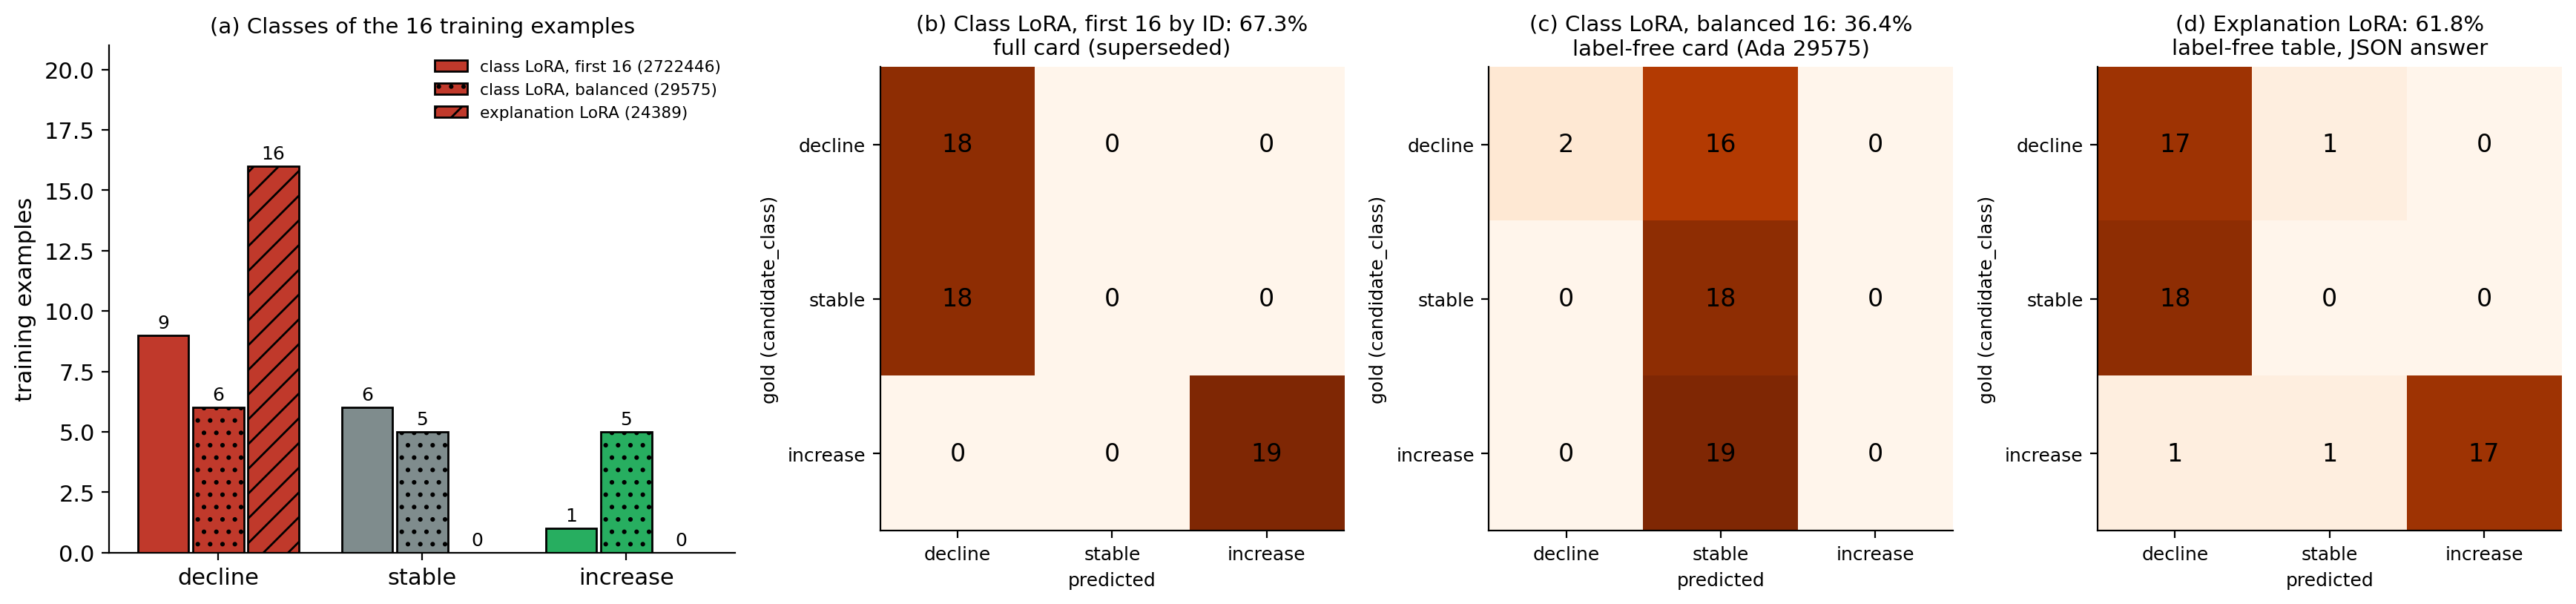
\includegraphics[width=\textwidth]{figures/fig_lora_v3.png}
\caption{All three LoRA runs. (a) Classes of the 16 training examples. (b) The first class LoRA (first 16 patches by ID, full card): 67.3\,\%, superseded. (c) The balanced, leak-free class LoRA: 36.4\,\%. (d) The explanation LoRA (Chapter~\ref{ch:trackC}). Made by \file{study_guide_v3/make_figures_v3.py}.}
\label{fig:loraclasses}
\end{figure}

\section{The first run, now superseded (Ada job 2722446)}

The first class LoRA (29 September, \texttt{--max-train 16 --epochs 1}) used the full card at training and test, and its 16 patches were simply the first 16 training patches by ID: 9 decline, 6 stable and 1 increase. It reached \textbf{67.3\,\%} (37/55): all decline and all increase patches right, every stable patch called ``decline'' (Figure~\ref{fig:loraclasses}b). It recognised all 19 increase patches from a single increase example, including 10 whose card trend word says ``stable'': on those cards only the \dndvi{} numbers and the summary line's \texttt{candidate\_class=increase} say ``increase''. Set beside job 29575, the likeliest reading is that it learned to use the label line.

\begin{newinfo}
Cite 36.4\,\% as your class-LoRA result. Keep 67.3\,\% only in an appendix or a single sentence, described as ``an earlier run on 16 unbalanced patches with the full card, which contains the label line''. Do not call it a leak-free or balanced result.
\end{newinfo}

\section{All fine-tuning jobs}

\begin{table}[H]
\centering
\caption{Every class-LoRA job whose log was copied back (\file{ada_review/EcoExplain-VLM-results/slurm-qwen09-*.log}, \file{results/slurm-qwen-balanced-smoke-29575.log}). Job 2722478 planned 3 epochs and its log ends after the first (loss 0.13); job 2792 stopped early after 2 epochs; jobs 2984 and 3054 had development accuracy 34.5\,\%. Job 2856 left an empty log. An earlier balanced job (29571) also finished; your notes name 29575 as the final artifact, and only its log is in the project.}
\label{tab:ftruns}
\small
\begin{tabular}{llrrlrr}
\toprule
Job & Date & Train & Epochs & Input (train / test) & Final loss & Test acc. \\
\midrule
\textbf{29575 (reported)} & 20 Oct & 16 bal. & 1 & label-free / label-free & 2.73 & \textbf{36.4\,\%} \\
2722446 (superseded) & 29 Sep & 16 by ID & 1 & full card / full card & 1.84 & 67.3\,\% \\
2722478 & 29 Sep & 256 & 1 of 3 & full card / --- & 0.13 & log ends \\
2690 & 2 Oct & 256 & 3 & full card / full card & 0.0000 & 100\,\% \\
2792 & 2 Oct & 256 & 2 & full card / full card & 0.0001 & 100\,\% \\
2984 & 2 Oct & 128 & 1 & full card / images only & 0.87 & 32.7\,\% \\
3054 & 2 Oct & 128 & 1 & full card / images only & 0.91 & 32.7\,\% \\
\bottomrule
\end{tabular}
\end{table}

\begin{itemize}
  \item \textbf{Jobs 2690 and 2792 reached 100\,\%} with almost zero training loss: with 256 examples and the full card, the model learned that the answer is written in the card's last line. Excluded.
  \item \textbf{Jobs 2984 and 3054} were trained with the card and tested on images alone: 32.7\,\%. Training and test inputs differ, so this is not a clean measurement.
  \item \textbf{Job 29575} is the first run in which training and test both lack the label line and the training classes are balanced. It is the only class-LoRA number that measures what the research question asks.
\end{itemize}

\begin{whybox}
Why still only 16 patches and one epoch? Job 29575 repeats the size of the first run so that the two differ only in balance and input, and it fits Ada's quota and queue. The natural next step is the configuration already scripted in \file{docs/PROTOCOL_RERUN.md}: 48 balanced patches (16 per class), or all 256, with the label-free card and early stopping on the development set.
\end{whybox}

\section{What you can and cannot claim}

\begin{table}[H]
\centering
\small
\begin{tabularx}{\textwidth}{YY}
\toprule
\textbf{You can say} & \textbf{You should not say} \\
\midrule
A LoRA on 16 balanced patches for one epoch, without the label line, reached 36.4\,\%, answering ``stable'' for 53 of 55 patches. & ``Fine-tuning improved the model to 67.3\,\%.'' \\
This is not better than always guessing one class ($p = 1.0$). & ``LoRA fixed the model's weaknesses.'' \\
An earlier unbalanced run with the full card reached 67.3\,\%, and longer full-card runs 100\,\%, because the card states the label. & ``The model reached 100\,\% after more training.'' \\
Larger, balanced, label-free fine-tuning remains untested. & ``Fine-tuning does not work for this task'' (16 examples cannot show that). \\
\bottomrule
\end{tabularx}
\end{table}

\begin{foryourreport}
In ``Effect of Fine-Tuning'' (about 400 words):
\begin{itemize}
  \item The configuration (Table~\ref{tab:classlora}), including the 6/5/5 balanced sample and the label-free card.
  \item 36.4\,\% with its interval, the per-class pattern (``stable'' for 53 of 55) and the McNemar tests.
  \item The earlier 67.3\,\% and 100\,\% runs in two sentences, as the reason the protocol was changed; Table~\ref{tab:ftruns} in an appendix.
  \item What would be needed next (more balanced patches, early stopping).
\end{itemize}
\end{foryourreport}

\begin{selfcheck}
\begin{enumerate}
  \item How did the training data and the input of job 29575 differ from those of job 2722446?
  \item What did the balanced, leak-free adapter answer, and why is 36.4\,\% not evidence of learning?
  \item Why is 67.3\,\% no longer the result to cite?
  \item What do jobs 2690 and 2792 show, and why are they excluded?
  \item What experiment would test fine-tuning properly?
\end{enumerate}
\end{selfcheck}
